\documentclass[10pt, conference, compsocconf]{IEEEtran}


\let\labelindent\relax

\usepackage{enumitem}
\usepackage[utf8]{inputenc}
\usepackage{color}
\usepackage{soul}
\usepackage{algorithmicx}
\usepackage{graphicx}
\usepackage{amssymb}
\usepackage{amsmath}
\usepackage{xspace}
\usepackage{algorithm}
\usepackage[noend]{algpseudocode}
\usepackage{subcaption}
\usepackage{float}
\usepackage{cite}
\usepackage{multirow}
\usepackage{flushend}



\everypar{\looseness=-1}

\newcommand{\mcomment}[1]{{\color{blue}{{\bf{mstf: }}#1}}}
\newcommand{\fcomment}[1]{{\color{green}{{\bf{fth: }}#1}}}
\newcommand{\kcomment}[1]{{\color{magenta}{{\bf{krm: }}#1}}}

\let\OLDthebibliography\thebibliography
\renewcommand\thebibliography[1]{
	\OLDthebibliography{#1}
	\setlength{\parskip}{0pt}
	\setlength{\itemsep}{0pt plus 0.3ex}
}

\floatname{algorithm}{Algorithm}
\renewcommand{\algorithmicrequire}{\textbf{Input:}}
\renewcommand{\algorithmicensure}{\textbf{Output:}}

\newcommand{\vtxs}{{\tt vtxs}}
\newcommand{\nbor}{{\tt nbor}}
\newcommand{\nets}{{\tt nets}}

\newcommand{\CP}{{\tt ColPack}\xspace}

\newcommand{\todo}[1]{\color{red}\textbf{\hl{\{ #1 \}}}\color{black}\xspace}

\usepackage{algorithm}
\usepackage{algpseudocode}
\usepackage{pbox}

\newtheorem{lemma}{\noindent Lemma}

% correct bad hyphenation here
\hyphenation{op-tical net-works semi-conduc-tor}

    
	\title{Parallel Count-Min Sketch on Multicores}
	
\author{\IEEEauthorblockN{Fatih Ta\c{s}yaran, Kerem Y{\i}ld{\i}r{\i}r, Mustafa Kemal Ta\c{s} and
Kamer Kaya} \vspace*{1ex}
\IEEEauthorblockA{Faculty of Engineering and Natural Sciences,\\
Computer Science and Engineering\\
Sabanc{\i} University, Turkey\\ \vspace*{2ex}
E-mail: {\small {\tt \{fatihtasyaran, keremyildirir, mkemaltas, kaya\}}}@sabanciuniv.edu}
}


	
\begin{document}

	\maketitle
    \begin{abstract}
   % One of the biggest challenges in today's business and technology world is dealing with enormous chunks of data. Many problems fail to scale up to large scales as their memory and time requirements are too high to produce exact results. %One of the problems
   % people encounter while working with big data is that it takes too much time to analyze it. 
   %Standard data structures like linked-lists
    %or hash tables are incompetent or inefficient for problems such as keeping track of the elements' frequency, or 
    %checking if an element is in the set or not. Hence, people are trying to come up with clever solutions such as data sketches. Data sketches are probabilistic data structures that give approximate results within mathematically proven error bounds while having orders of magnitude less memory and time complexities than traditional approaches. Hence they are ideal for architectures with limited memory and computation power such as {\tt Raspberry Pi}.
    %In this paper, we propose methods for adapting Count-Min Sketch to Raspberry Pi architectures. Also, we propose various optimizations to increase the efficiency without decreasing the accuracy of the algorithm.

One of the biggest challenges today is analyzing enormous chunks of data gathered from different sources. Traditional approaches for data analysis fail to scale as their memory and time requirement are too high to be practical.
% Standard data structures such as counters or hash tables can be inefficient while answering problems such as frequency analysis or set membership. 
Sketches are probabilistic data structures that can provide approximate results within mathematically proven error bounds while having orders of magnitude less memory and time complexities than traditional approaches. Hence, they can be employed for big data analysis by architectures even with limited memory such as a {\tt Raspberry Pi}. Today, such architectures usually offer multiple cores. With efficient parallel sketching, they can manage high volumes of data streams and be utilized for edge computing. For instance, a single Raspberry Pi deployed at the edge of a network can perform frequency analysis on streaming data obtained by many IoT sensors.

In this work, we provide a parallel implementation for Count-Min Sketch which has been frequently used for various applications. We evaluate its performance both on a high-end server and a Raspberry Pi. We used tabulation hashing and to obtain a parallel and cache friendly implementation, we combine the tables for different hash functions in an alternating way. The results are promising as they show that the proposed implementation can be applied to improve the amount of real-time streaming data managed by single board computers and higher-end servers with multiple cores.    
    	
    
\end{abstract}
    \section{Introduction}
    
   Today, many applications such as financial markets~\cite{chandramouli2010} and network traffic analysis~\cite{fan1998,duffield2001} has a streaming nature. For these applications, the data can rapidly scale up to massive amounts, making them impossible to store and allowing only a single pass over the stream.  Furthermore, since the data arrive at real-time, it may be impractical to process it and answer the queries, such as membership~\cite{brodnik1999} and/or frequency~\cite{charikar2002}, with 100$\%$ accuracy. Although exact computation can be possible for slower streams by processing the data on cutting-edge servers equipped with a large memory and powerful processor(s), enabling less power hungry devices such as single-board computers, e.g., Raspberry Pi, Odroid etc., with smarter algorithms and data structures yields much energy efficient and cheaper solutions for the same task. A comprehensive survey of data stream applications can be found in~\cite{muthukrishnan2005}. 
      
Sketching is a probabilistic data summarization technique; there exist various sketches in the literature tailored for different applications. These data structures can work on streaming data and help us to process a query with small, even sub-linear, amount of memory for many problems~\cite{alon1996,charikar2002,dobra2002,gilbert2002}. Furthermore, sketches are very useful for distributed data streams since each stream can independently be sketched and then these sketches can be combined to obtain the final sketch. To remove the bias on the data distribution, sketches frequently employ hashing. This maps the actual data to datasets on which various statistical analysis can be performed for problems such as heavy-hitters, count distinct, rare counts etc. Due to the implicit compression being performed during this process, there is almost always a trade-off between the accuracy of the final result and the size of the sketch. A complete analysis and comparison of various sketches can be found in~\cite{cormode2005}.
	  
As stated above, sketches are tailored for different applications; one of the most popular and well-known sketches today is {\it Bloom Filter}~\cite{bloom1970} which is designed to answer membership queries. Despite allowing false-positives, i.e. falsely confirming the existence of a non-existent item, Bloom Filters have proven to be useful for many applications employing membership queries~\cite{broder2002}. However, they fail to perform any kind of counting the frequencies of the items. Thus, a more sophisticated data structure is required.

{\it Count-Min Sketch}~(CMS) is probabilistic sketch that helps to estimate the frequencies, i.e., the number of occurrences, of distinct items in a stream~\cite{cormode2005}. The frequency  information is crucial to find finding heavy-hitters or rare items or detecting anomalies within a large computer network~\cite{cormode2003, cormode2005}. Unlike Bloom Filters which use bits, CMSs store a small counter table to keep track of the frequency of each distinct element. Intuitively, the reduction to sub-linear space decreases the accuracy in the sense that the frequencies of some elements can be overestimated due to the collisions of hash functions. An important property of a CMS is that the error is always one sided; that is, the sketch never underestimates the frequencies. 

In this work, we focus on multicore implementation of Count-Min sketches and experiment both on a high-end server and a Raspberry Pi. As hashing function, we used {\em tabulation hashing} which is simple and provide unexpectedly strong statistical guarantees~\cite{patrascu2012,thorup2017}. Our first contribution is designing a cache-friendly implementation to compute multiple tabulation hashes at a time which is a crucial operation for CMS. The proposed approach can be useful not only for CMS but also other applications that needs to hash the same element multiple times which is a common operation in many sketches. We then restructure the CMS construction in a way to process the data stream in parallel while avoiding possible race-conditions on a single CMS table as much as possible. An efficient synchronization mechanism is necessary since race-conditions can both decrease the performance and also increase the amount of error estimated by statistical analysis by taking the table size into account. 

The  rest of the article is organized as follows: Section~\ref{sec:not} presents the background and describes the notation that will be used later. In Sections~\ref{sec:tab} and~\ref{sec:par}, the cache-friendly tabular hashing mechanism and corresponding parallel CMS construction implementation will be proposed. Section~\ref{sec:exp} presents the experimental results and Section~\ref{sec:con} concludes the paper.
   
 \section{Notation and Background}\label{sec:not}

Let ${\cal U} = \{1,\cdots,n\}$ be the universal set where the elements in the stream are coming from. 
Let $N$ be size of the stream ${\tt s}[.]$ where ${\tt s}[i]$ denotes the $i$th element in the stream.
We will use $f_x$ to denote the frequency of an item. Hence, $$f_x = |\{x = {\tt s}[i]: 1 \leq i \leq N\}|.$$

Given two parameters $\epsilon$ and $\delta$, a Count-Min Sketch is constructed as a two-dimensional counter array with 
$d = \lceil \ln(1/\delta) \rceil$ rows and $w = \lceil e/\epsilon \rceil$ columns. 
There are two fundamental operations for a CMS; the first one is {\em insert}($x$) which is used to construct/update 
the internal sketch counters to insert an item $x \in {\cal U}$. Initially, all the counters inside the sketch are set to $0$. 
To insert an item $x \in {\cal U}$, for $1 \leq i \leq d$, the counters ${\tt cms}[i][h_i(x)]$ are incremented. Figure~\ref{fig:cms_insert} illustrates a single insertion and Algorithm~\ref{alg:cms_construct} gives the pre the process of processing a stream ${\tt s}[.]$ of size $N$. 

 \begin{figure}[htbp]
\begin{center}
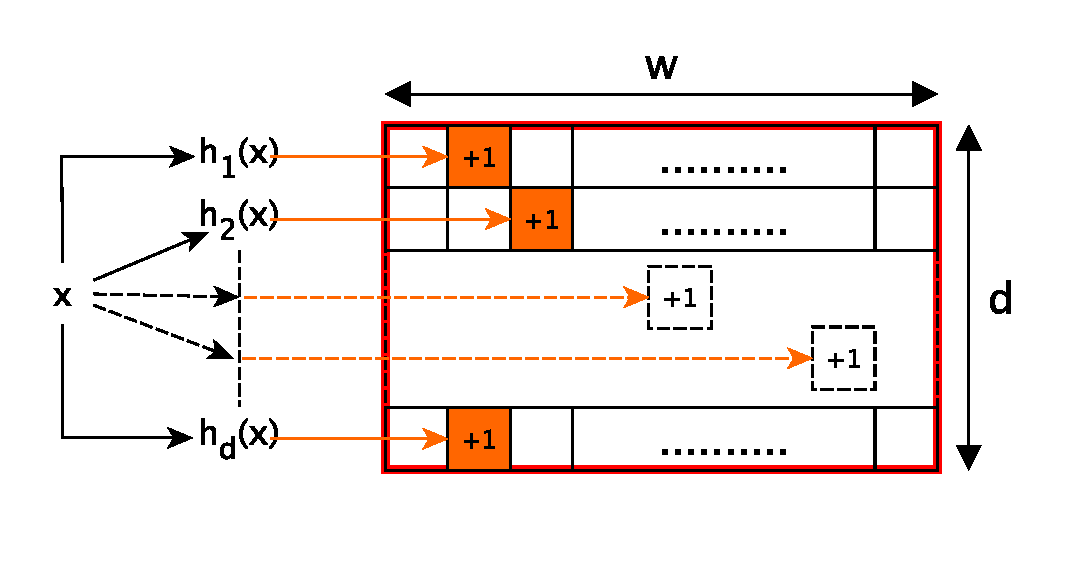
\includegraphics[width=0.90\linewidth]{cms.pdf}
\caption{Illustration of the insert operation for Count-Min Sketch}
\label{fig:cms_insert}
\end{center}
\end{figure}
 
 \begin{algorithm}[htbp]
  	\small
  	\caption{\textsc{CMS-Construction}} 
  	\algorithmicrequire{  $\epsilon$: error factor\\
	 		\hspace*{6ex} $\delta$: error probability \\
	 	  \hspace*{7ex}${\tt s}[.]$: a stream with $N$ elements from $n$ distinct elements \\ 
		  \hspace*{7ex}$h_i(.)$: pairwise independent hash functions where for \\ 
		  \hspace*{13ex}$1\leq i \leq d$,  $h_i$: ${\cal U} \rightarrow \{1,\cdots,w\}$ and $w = \lceil e/\epsilon \rceil$\\ \\}
	 \algorithmicensure{ ${\tt cms}[.][.]$: a $d \times w$ counter sketch where $d = \lceil 1/\delta \rceil$ \\
	 }
  	\begin{algorithmic}[1]
		\For{$i$ from $1$ to $d$}
			\For{$j$ from $1$ to $w$}
				\State{${\tt cms}$[i][j] $ \leftarrow 0$}
			\EndFor
		\EndFor
		\For{$i$ from $1$ to $N$}
			\State $x  \leftarrow s[i]$
			\For{$j$ from $1$ to $d$}
				\State {$col \leftarrow h_j(x)$} 
				\State{${\tt cms}$[j][$col$] $ \leftarrow {\tt cms}$[j][$col$] $ +1$}
			\EndFor
		\EndFor
	\end{algorithmic}
	\label{alg:cms_construct}
\end{algorithm} 	

 
The second operation for CMS is {\em query}($x$) which estimates the frequency of $x \in {\cal U}$ as $$f'_x = min_{1 \leq i \leq d}\{{\tt cms}[i][h_i(x)]\}.$$
\noindent With $d \times w$ memory, the sketch satisfies that
 $f_x \leq f'_x$ and $f'_x \leq f_x + \epsilon N$ with probability at least $1 - \delta$. Hence, the error is always one-sided, i.e., the
 estimation is always larger than the actual frequency. Furthermore, the error is additive, and for $\epsilon$ and $\delta$ small enough, the amount of the error 
 is also small w.h.p. especially if $f_x$  is large, i.e., $x$ is a frequent item. 

\subsection{Tabulation Hashing}

CMS uses pairwise independent hash functions to provide the desired properties stated above. There exist a separate hash function for each row of the CMS with a range equal 
to the range of columns. In this work, we use Tabulation Hashing~\cite{zobrist1970} which has been recently analyzed by Patrascu and Thorup et al.~\cite{patrascu2012,thorup2017} and shown to provide unexpectedly strong guarantees despite of its simplicity. Furthermore, it has been shown that even a slightly more sophisticated version of tabulation hashing is almost as fast as the classic multiply-mod-prime scheme, i.e., $(ax + b) \bmod p$. 

Assuming each element in {\cal U} is represented in 32 bits and the desired output is also 32 bits, the tabulation hashing works as follows: first a $4 \times 256$ table is generated and filled with random 32-bit values. Given a 32-bit input $x$, each character, i.e., 8-bit value, of $x$ is used as an index for the corresponding row. Hence, four 32-bit values, one from each row, are extracted from the table. The {\tt XOR} of these 32-bit values are returned as the hash value. The implementation we use in this work is given in Figure~\ref{fig:tabulation_seq}.

\begin{figure}[htbp]
\begin{center}
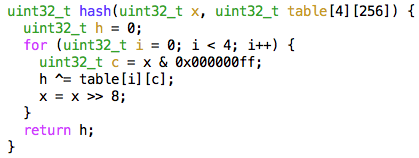
\includegraphics[width=0.90\linewidth]{tabular_code.png}
\caption{Naive tabulation hashing in C++}
\label{fig:tabulation_seq}
\end{center}
\end{figure}

\section{Multiple Tabulation Hashes at Once}\label{sec:tab}

Although the auxiliary data used in tabulation hashing are usually small and can fit into a cache, the spatial locality of the accessed elements in the tables are not cache friendly since each access is performed to a different table row. A naive, cache-friendly rearrangement of the entries in the table is also not possible for applications performing a single hash per item; the indices for the table rows are obtained from adjacent chunks in the binary representation of the hashed item whose decimal values are usually not correlated hence there is no relation whatsoever among them to help us to fix the access pattern.

In addition to CMS, for many frequency sketches, e.g., Count Sketch~\cite{charikar2002} and Count-Mean-Min Sketch~\cite{Goyal2012}, the same item is hashed more than once. For tabulation hashing, this yields an interesting optimization; there exist multiple hash functions and hence more than one hash table. Although, a single table is still accessed in an irregular fashion, the accessed coordinates in all the tables are the same for different tables. This can be observed on the left side of Figure~\ref{fig:merged_tabular_access}. Hence, the columns of the tables can be combined in an alternating fashion as shown in the right side of the figure. In this approach, when only a single thread is responsible from inserting the appearance of a single item to CMS, the cache can be utilized in a better way. This is called {\em merged tabulation}.

 \begin{figure}[htbp]
\begin{center}
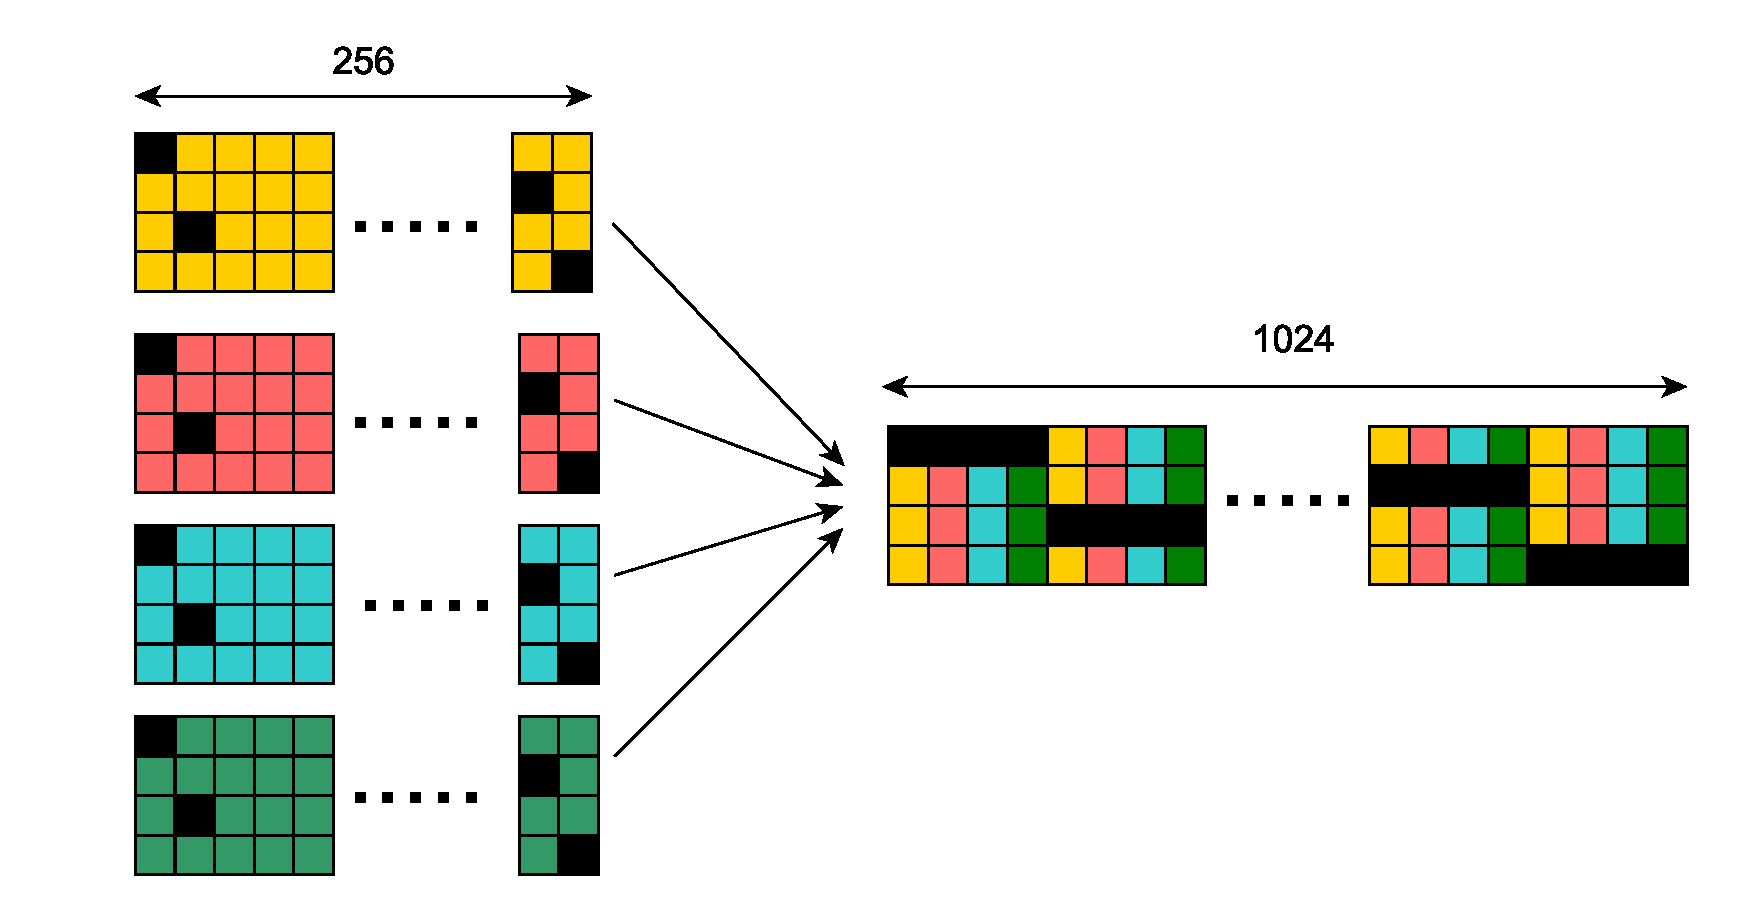
\includegraphics[width=0.96\linewidth]{merged_tabular_access.pdf}
\caption{Memory access patterns for naive and merged tabulation for four hashes. The hash tables are colored with different colors. The accessed locations for both approaches are shown in black.}
\label{fig:merged_tabular_access}
\end{center}
\end{figure}

With merged tabulation, the consecutive elements in the merged table belong to different hash values. Since these values require multiple {\tt XOR} operations, we need to store the partial results in the memory. A simple C++ implementation of merged tabulation which uses a single $4 \times 1024$ table to compute four hashes at once is given in Figure~\ref{fig:tabulation_merged}.

\begin{figure}[htbp]
\begin{center}
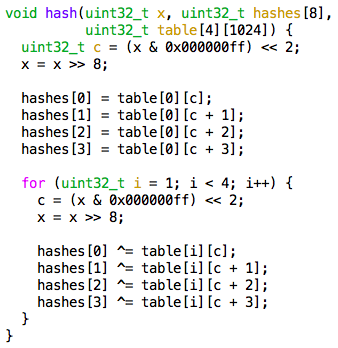
\includegraphics[width=0.75\linewidth]{tabular_code_par}
\caption{Merged tabulation hashing implementation in C++}
\label{fig:tabulation_merged}
\end{center}
\end{figure}

\section{Parallel Count-Min Sketch Construction}\label{sec:par}

Since multiple CMS sketches can be combined, on a multicore hardware,  each thread can process a different part of the data (with the same hash functions) to construct a partial CMS. These partial sketches can then be aggregated by adding the counter values in the same locations  to obtain the final value on the combined CMS sketch. Although this approach requires no synchronization until all partial sketches are constructed, compared to constructing the final CMS table directly, it consumes more memory. Furthermore, the amount of the memory is increasing with increasing number of threads. 

Constructing a single CMS sketch in parallel is not a straightforward task. The pseudocode of the naive parallel CMS construction is given in Algorithm~\ref{alg:cms_construct_par_nobuf}. When a thread processes a single data item, it accesses an arbitrary column of each CMS row. Hence, race conditions may reduce the estimation accuracy. In addition, these memory accesses are a probable cause of false sharing which prevents the implementation to utilize the hardware to its full potential. To avoid the pitfalls stated above, one could assign each item to multiple threads which evaluate different hash functions hence touch different rows of the CMS table. However, this approach cannot use the merged tabulation since, each thread performs only a single hash of an item. 


 \begin{algorithm}[htbp]
  	\small
  	\caption{\textsc{Naive-Parallel-CMS}} 
  	\algorithmicrequire{  $\epsilon$: error factor\\
	 		\hspace*{6ex} $\delta$: error probability \\
	 	  \hspace*{7ex}${\tt s}[.]$: a stream with $N$ elements from $n$ distinct elements \\ 
		  \hspace*{7ex}$h_i(.)$: pairwise independent hash functions where for \\ 
		  \hspace*{13ex}$1\leq i \leq d$,  $h_i$: ${\cal U} \rightarrow \{1,\cdots,w\}$ and $w = \lceil e/\epsilon \rceil$\\
		  \hspace*{7ex}$\tau$: no threads\\ }
	 \algorithmicensure{ ${\tt cms}[.][.]$: a $d \times w$ counter sketch where $d = \lceil 1/\delta \rceil$ \\
	 }
  	\begin{algorithmic}[1]
		\State{Reset all the ${\tt cms}[.][.]$ counters to 0 (as in Algorithm~\ref{alg:cms_construct}).}
		\State{}
		
		\For{$i$ from $1$ to $N$ {\bf in parallel}}
			\State $x  \leftarrow s[i]$
			\State ${\tt hashes}[.] \leftarrow$ {\sc MergedHash}($x$)

			\For{$j$ from $1$ to $d$}
				\State {$col \leftarrow {\tt hashes}[j] $} 
				\State{${\tt cms}$[j][$col$] $ \leftarrow {\tt cms}$[j][$col$] $ +1$}
			\EndFor
		\EndFor
	\end{algorithmic}
	\label{alg:cms_construct_par_nobuf}
\end{algorithm} 	

In this work, we propose a {\em buffered parallel} execution to alleviate the above mentioned issues; we (1) divide the data into batches and (2) process a single batch in parallel in two stages; a) hashing and b) CMS counter updates. In the proposed approach, after each batch, the threads synchronize and process the next one. For batches with $b$ elements, the first stage requires a buffer of size $b \times d$ to store the hash values, i.e., column ids, which then will be used in the second stage to update CMS counters. Such a buffer allows us to use merged tabulation effectively during the first stage. For the second stage, we used at most $d$ threads. In our implementation, the counters in a row are updated by the same thread hence, there will be no race conditions and probably much less false sharing. We also experiment with extra padding between the table rows which we found to be useful for CMS tables with a small $w$ value. Algorithm~\ref{alg:cms_construct_par} gives the pseudocode for our CMS construction approach.

 \begin{algorithm}[htbp]
  	\small
  	\caption{\textsc{Buffered-Parallel-CMS}} 
  	\algorithmicrequire{  $\epsilon$: error factor\\
	 		\hspace*{6ex} $\delta$: error probability \\
	 	  \hspace*{7ex}${\tt s}[.]$: a stream with $N$ elements from $n$ distinct elements \\ 
		  \hspace*{7ex}$h_i(.)$: pairwise independent hash functions where for \\ 
		  \hspace*{13ex}$1\leq i \leq d$,  $h_i$: ${\cal U} \rightarrow \{1,\cdots,w\}$ and $w = \lceil e/\epsilon \rceil$\\
		  \hspace*{7ex}$b$: batch size (assumption: divides $N$)\\
		  \hspace*{7ex}$\tau$: no threads (assumption: divides $d$)\\ }
	 \algorithmicensure{ ${\tt cms}[.][.]$: a $d \times w$ counter sketch where $d = \lceil 1/\delta \rceil$ \\
	 }
  	\begin{algorithmic}[1]
		\State{Reset all the ${\tt cms}[.][.]$ counters to 0 (as in Algorithm~\ref{alg:cms_construct}).}
		\State{}
		
		\For{$i$ from $1$ to $N/b$}
			\State $j_{end} \leftarrow i \times b$	 \Comment{\bf Stage 1}
			\State $j_{start} \leftarrow j_{end} - b + 1$
			
			\For{$j$ from $j_{start}$ to $j_{end}$ {\bf in parallel}}
				\State $x  \leftarrow {\tt s}[j]$
				\State $\ell_{end} \leftarrow j \times d$
				\State $\ell_{start} \leftarrow \ell_{end} - d + 1$
				\State ${\tt buf}[\ell_{start}, \cdots, \ell_{end}] \leftarrow$ {\sc MergedHash}($x$)
			\EndFor
			
			
			\For{$t_{id}$ from $1$ to $\tau$ {\bf in parallel}} \Comment{\bf Stage 2}
				\For{$j$ from $1$ to $b$ }
					\State{$nrows \leftarrow d / \tau$}
					\State $r_{end} \leftarrow t_{id} \times nrows$
					\State $r_{start} \leftarrow r_{end} - nrows + 1$
					\For{$r$ from $r_{start}$ to $r_{end}$ }
						\State{$col \leftarrow {\tt buf}[((j-1) \times d) + r]$}
						\State{${\tt cms}[r][col] \leftarrow {\tt cms}[r][col] +1$}
					\EndFor
				\EndFor
			\EndFor

			
		\EndFor
	\end{algorithmic}
	\label{alg:cms_construct_par}
\end{algorithm} 	

\section{Experimental Results}\label{sec:exp}

To understand the performance of the proposed approach, we perform the experiments on two architectures:  {\bf Arch-1} is a server running on 64 bit CentOS 6.5 equipped with 64GB RAM and a dual-socket Intel Xeon E7-4870 v2 clocked at 2.30 GHz where each socket has 15 cores~(30 in total). {\bf Arch-2} is a quad-core 64-bit ARM Cortex A53 clocked at 1.2 GHz equipped with 1 GB LPDDR2-900 SDRAM. It is running on Raspbian GNU/Linux 9. For the multicore implementations, we use C++11 and OpenMP. We use {\tt gcc 5.3.0} with the {\tt -O3} optimization flag enabled on {\bf Arch-1}. On {\bf Arch-2} the compiler is {\tt gcc 6.3.0} and the {\tt -O3} optimization flag is enabled.

To generate the datasets used in the experiments, we used a {\em Zipfian} distribution. Although this study focuses on the performance which is not directly related to the distribution of the values in the stream ${\tt s}[.]$, many data in real world such as number of paper citations, file transfer sizes, word frequencies etc. fit to a Zipfian distribution. Furthermore, although the statistical analysis for CMS do not depend on the data, Zipfian is a common choice for the studies in the literature to benchmark the estimation accuracy of data sketches. We used the shape parameter $\alpha = 0.9$ to generate the distribution. 

We employ two sets of $(\epsilon, \delta)$ values to generate CMS tables; in the first one, we used $(\epsilon = 0.01, \delta = 0.003)$ to generate a {\bf small} sketch with $d = \lceil \log_2(1/\delta) \rceil = 8$ and $w = 211$ where $w$ is selected as the first prime after $2/\epsilon$. In addition, we generate a relatively {\bf large} sketch with $(\epsilon = 0.01, \delta = 0.003)$ with $d = 8$ rows and $w = 2003$ columns.


For the experiments on {\bf Arch-1}, we choose $N = 2^{30}$ elements from a universal set $\cal U$ of cardinality $n = 2^{25}$. For {\bf Arch-2}, i.e., Raspberry Pi, we use $N = 2^{25}$ and $n = 2^{20}$. We used $b = 1024$ as the batch size. Each data point in the tables and charts given below is obtained by averaging ten consecutive runs. 

\subsection{Parallel CMS construction with partial sketches}

In the first set of experiments, we measure the performance improvement due to merged tabulation in the partial sketches setting. That is, each thread is responsible from a different part of the stream and construct a partial sketch for that part. Hence, no synchronization mechanism is required since all these constructions are independent from each other. The results of this set of experiments are given in Table~\ref{tbl:mergedtbl}. 

\begin{table*}[htbp]
\centering
{\def\arraystretch{1.3}
\begin{tabular}{ccccc||ccccc|ccccc}  
                                 &&&&                 & \multicolumn{5}{c|}{\textbf{Naive Tabulation}} & \multicolumn{5}{c}{\textbf{Merged Tabulation}} \\
                                   &&&&                 & $\tau$=1   & $\tau$=2    & $\tau$=4    & $\tau$=8    & $\tau$=16  & $\tau$=1   & $\tau$=2   & $\tau$=4   & $\tau$=8   & $\tau$=16 \\ \hline
                                   

\multicolumn{1}{l}{\multirow{4}{*}{\textbf{Zipf 0.9}}}
&&&\multirow{2}{*}{\textbf{Arch-1}} & \textbf{small}  & 63.9    & 40.8   & 25.4   & 14.4   & 7.5   & 61.1    & 34.0    & 17.4   & 9.5   & 5.1   \\
                                 &&&& \textbf{large} & 67.6    & 34.1   & 19.2   &   9.5 & 4.9   &  60.4 &	33.7 &	17.3	& 8.9	& 4.4 \\ \cline{2-15}
             
&&&\multirow{2}{*}{\textbf{Arch-2}} & \textbf{small}  & 31.6    & 15.9   & 8.2   &        &       &  28.6    &  14.3   & 7.3   &        &       \\
                                 &&&& \textbf{large} &  32.8      &   16.5     &       8.3 &        &       &     30.8    &     15.4    &     7.7   &        &   \\ \hline  
\multicolumn{1}{l}{\multirow{4}{*}{\textbf{Zipf 1.1}}}
&&&\multirow{2}{*}{\textbf{Arch-1}} & \textbf{small}  & 65.8    & 32.2   & 19.6   & 11.9   & 6.1   & 60.0    & 33.1    & 16.6   & 9.0   & 4.8   \\
&&&& \textbf{large} & 65.7    & 33.2   & 18.4   &   9.4 & 4.6   &  60.0 &	32.5 &	16.8	& 8.4	& 4.2 \\ \cline{2-15}

&&&\multirow{2}{*}{\textbf{Arch-2}} & \textbf{small}  & 31.5    & 15.9   & 8.4   &        &       &  28.8    &  14.6   & 7.5   &        &       \\
&&&& \textbf{large} &  32.4      &   16.1     &       10.1 &        &       &     29.6    &     15.0    &     8.9   &        &   \\ \hline 
\multicolumn{1}{l}{\multirow{4}{*}{\textbf{Zipf 1.5}}}
&&&\multirow{2}{*}{\textbf{Arch-1}} & \textbf{small}  & 63.2    & 32.7   & 17.8   & 10.6   & 5.7   & 59.7    & 30.7    & 15.4   & 7.9   & 4.0   \\
&&&& \textbf{large} & 63.8    & 32.0   & 16.3   &   8.2 & 4.1   &  59.7 &	30.3 &	15.3	& 7.6	& 3.8 \\ \cline{2-15}

&&&\multirow{2}{*}{\textbf{Arch-2}} & \textbf{small}  & 31.1    & 15.7   & 8.0   &        &       &  28.6    &  14.4   & 7.4   &        &       \\
&&&& \textbf{large} &  30.9      &   15.5     &      7.8 &        &       &     28.3    &     14.3    &     7.2   &        &   \\ \hline   
\multicolumn{1}{l}{\multirow{4}{*}{\textbf{Zipf 2}}}
&&&\multirow{2}{*}{\textbf{Arch-1}} & \textbf{small}  & 67.8    & 32.8   & 17.1   & 9.1   & 4.3   & 59.8    & 30.3    & 15.1   & 7.7   & 3.9   \\
&&&& \textbf{large} & 63.0    & 31.6   & 16.0   &  7.9 & 4.0   &  59.8 &	30.0&	15.0	& 7.5	& 3.7 \\ \cline{2-15}

&&&\multirow{2}{*}{\textbf{Arch-2}} & \textbf{small}  & 31.1    & 15.6   & 8.5   &        &       &  28.8    &  14.8   & 8.0   &        &       \\
&&&& \textbf{large} &  31.1      &   15.5     &   9.5 &        &       &     28.2    &     14.3    &     8.9   &        &   \\ \hline
\multicolumn{1}{l}{\multirow{4}{*}{\textbf{Zipf 3}}}
&&&\multirow{2}{*}{\textbf{Arch-1}} & \textbf{small}  & 62.9    & 31.9   & 16.4   & 8.3   & 4.2   & 59.8    & 29.9    & 14.9   & 7.5   & 3.7   \\
&&&& \textbf{large} & 63.0    & 31.5   & 15.7   &  7.9 & 3.9   &  60.0 &	29.9&	15.0	& 7.5	& 3.7 \\ \cline{2-15}

&&&\multirow{2}{*}{\textbf{Arch-2}} & \textbf{small}  & 31.0    & 15.8   & 8.3   &        &       &  28.7    &  14.6   & 7.4   &        &       \\
&&&& \textbf{large} &  31.2      &   15.5     &   9.8 &        &       &    28.4    &     14.4    &     8.9   &        &   \\ \hline    
\multicolumn{1}{l}{\multirow{4}{*}{\textbf{Uniform}}}
&&&\multirow{2}{*}{\textbf{Arch-1}} & \textbf{small}  & 64.3    & 33.1   & 23.1   & 14.0   & 7.6   & 60.4    & 34.4    & 17.5   & 10.0   & 5.2   \\
&&&& \textbf{large} & 72.3    & 36.8   & 20.0   &   9.8 & 4.9   &  60.6 &	33.3 &	17.1	& 8.8	& 4.5 \\ \cline{2-15}

&&&\multirow{2}{*}{\textbf{Arch-2}} & \textbf{small}  & 31.8    & 16.0   & 8.0   &        &       &  28.3    &  14.2   & 7.1   &        &       \\
&&&& \textbf{large} &  33.2      &   16.7     &       8.44 &        &       &     30.8    &     15.4    &     7.75   &        &   \\ %\hline  
\end{tabular}
}
\caption{Parallel CMS construction times (in seconds) with naive and merged tabulation for $\tau \in \{1, 2, 4, 8, 16\}$ threads on \textbf{Arch-1} and  $\tau \in \{1, 2, 4\}$ threads on \textbf{Arch-2}. The stream sizes for \textbf{Arch-1} and \textbf{Arch-2} are $N = 2^{30}$ and $N = 2^{25}$, respectively. The rows labeled with {\bf small} and {\bf large} denote the $8 \times 211$ and $8 \times 2003$ CMS tables, respectively. } \label{tbl:mergedtbl}

\end{table*}

As the results in Table~\ref{tbl:mergedtbl} show, merged tabulation increases the performance of the CMS construction even with extra overhead of managing an auxiliary array, i.e., $\tt hashes[.]$ in Figure~\ref{fig:tabulation_merged}. Instead of using a single register as in naive tabulation shown in Figure~\ref{fig:tabulation_seq}, in merged tabulation, the intermediate hash values are first written to the auxiliary memory. Once all $d$ hashes are computed, they are read back from the memory again. However, these extra reads as well as the hash table accesses are more cache friendly.

The impact of merged tabulation in terms of improvement percentage behaves differently on {\bf Arch-1} and {\bf Arch-2} and for {\bf small} and {\bf large} sketches. On {\bf Arch-2}, the improvements on the CMS construction time with $\tau = 1$, $2$ and $4$ threads are $10.5\%$, $11\%$ and $12\%$ on {\bf small} sketches and $6.5\%$, $7\%$ and $8\%$ on {\bf large} sketches, respectively.  Hence, the amount of the improvement does not change with the number of threads and sketch sizes. On {\bf Arch-1}, the improvement starts with $4.5\%$ with a single thread for the {\bf small} sketch, merged tabulation increases the runtime by $2\%$ for two threads., with $\tau = 2$, $4$, $8$ and $16$, the improvement becomes $20\%$, $46\%$, $51\%$ and $47\%$, respectively. On the other hand, for the {\bf large} sketch, the improvement is more stable and in between $2\%$ and $12\%$ for varying number of threads.

The results show that a smaller sketch on {\bf Arch-1} can benefit from the merged tabulation better. We believe that this is due to the common cache lines among the last row and the first row of two partial sketches. With naive tabulation, a thread accesses to a partial sketch after each hash computation. Hence, the accesses are frequent  with short intervals in between. On the other hand, with merged tabulation, each $d$ consecutive accesses are combined, and in between, $d$ hash functions are computed. This reduces the probability of concurrent updates on the same cache line by two threads.  

\subsection{Parallel CMS construction with a single sketch}

Although using partial sketches is pleasingly parallelizable and can be practical for some use cases, it is not a good approach for memory restricted devices such as Raspberry Pi. The additional memory might be required by other applications running on the same hardware and/or other types of skeches being maintained at the same time for the same or a different data stream. This is why in the rest of the experiments, we focus on the single CMS sketch case. Similarly, we apply merged tabulation for all the implementation in the rest of the paper.  

Table~\ref{tbl:batch} shows the results of the experiments in which a single sketch is constructed in parallel. As expected, the naive parallel approach suffer from false sharing with multiple threads on {\bf Arch-1}. However, we did not observe the such a dramatic slowdown on {\bf Arch-2}. Furthermore, the improvement behaves differently on these two architectures. Since buffering the hashes has an overhead, we expect a slowdown in a sequential execution. This is what we observe on {\bf Arch-1}; the runtimes are increased to  68.9 and 68.6 seconds from 61.4 and
 60.4 seconds, respectively for {\bf small} and {\bf large} sketches. However, we do not see the same pattern on {\bf Arch-2}.
We believe this is due to the existence of a relatively smaller L1 cache on {\bf Arch-2} which is equipped with a 16KB L1 cache per core and a 512KB L2 cache per processor. On {\bf Arch-1}, we have 32KB L1, 256KB L2 caches per core and 30MB L3 cache per processor. In the naive parallel approach, locations in the merged hash table and in the sketch are accessed one after another in an alternating fashion. Hence, these structures need to live in the cache at the same time for efficiency. An advantage of the buffered parallel approach is that it separates the accesses to these structures. Hence, it does not use the cache for these structures at the same time. 

Overall, the buffered parallel approach is significantly better than the naive parallel one; it improves the runtimes and yields a better scalability. However, for the {\bf small} table on {\bf Arch-1}, the proposed approach yields much less parallel efficiency compared to the results of the {\bf large} sketch. This is expected since, with multiple threads performing simultaneous updates on the sketch, whose rows are stored consecutively on the memory, false sharing can reduce the performance. Furthermore, the impact will be more drastic for smaller $w$ values which is the case in our experiments. To avoid false sharing as much as possible, we added extra padding to each row of CMS sketch. The third set of columns in Table~\ref{tbl:batch} shows the execution times after padding. As the results confirm, padding helps to get rid of the problems arose from increased coherency traffic due to the concurrent updates on the same cache line by multiple threads. 

\begin{table*}[]
\centering

{\def\arraystretch{1.3}
\begin{tabular}{ccc||ccccc|ccccc|ccccc}
                                   &&                 & \multicolumn{5}{c|}{\textbf{Naive Parallel}} & \multicolumn{5}{c|}{\textbf{Buffered Parallel}} & \multicolumn{5}{c}{\textbf{Buffered Parallel with Padding}} \\
                                                                      &&                 & \multicolumn{5}{c|}{(Algorithm~\ref{alg:cms_construct_par_nobuf})} & \multicolumn{5}{c|}{(Algorithm~\ref{alg:cms_construct_par})} & \multicolumn{5}{c}{(Algorithm~\ref{alg:cms_construct_par} + Padding)} \\

                                   &&                 & $\tau$=1   & $\tau$=2    & $\tau$=4    & $\tau$=8    & $\tau$=16  & $\tau$=1   & $\tau$=2   & $\tau$=4   & $\tau$=8   & $\tau$=16  & $\tau$=1   & $\tau$=2   & $\tau$=4   & $\tau$=8   & $\tau$=16 \\ \hline
\multicolumn{1}{c}{\multirow{4}{*}{\textbf{Zipf 0.9}}} 
&\multirow{2}{*}{\textbf{Arch-1}} & \textbf{small}  & 61.4  & 289.8  & 287.0  & 176.6  & 118.3 & 68.0  & 61.9  & 45.0  & 29.7  & 27.2  & 68.3  & 46.7  & 24.4    & 13.6  & 10.9 \\
                                   && \textbf{large} & 60.4  & 240.0  & 225.3  & 137.2  & 96.9  & 68.6  & 50.3  & 28.2  & 15.8& 13.4&68.5&43.6&22.7&12.7& 10.4 \\ \cline{2-18}
&\multirow{2}{*}{\textbf{Arch-2}}  & \textbf{small}  & 28.7  & 15.4   & 7.7   &        &       & 27.7  & 13.8  & 7.4  &       &       & 27.8  & 13.8  & 7.5  &       &      \\
                                   && \textbf{large} & 30.7  & 15.4   & 7.7   &        &       & 26.8  & 13.3  & 8.3  &       &       & 27.2  & 13.3  & 8.3  &       &  \\ \hline 
 
\multicolumn{1}{c}{\multirow{4}{*}{\textbf{Zipf 1.1}}} 
&\multirow{2}{*}{\textbf{Arch-1}} & \textbf{small}  & 60.25  & 287.6  & 287.3  & 179.3  & 125.9 & 68.1  & 58.4  & 40.1  & 26.2  & 24.1  & 68.09  & 43.5  & 22.9    & 13.0  & 10.6 \\
&& \textbf{large} & 60.9  & 146.1  & 222.2  & 159.1  & 130.5  & 68.3  & 51.4  & 28.7  & 16.0& 13.2&68.4&46.4&24.3&13.6& 10.8 \\ \cline{2-18}
&\multirow{2}{*}{\textbf{Arch-2}}  & \textbf{small}  & 28.7  & 15.5   & 8.6   &        &       & 27.7  & 13.9  & 7.39  &       &       & 27.89  & 13.9  & 7.4  &       &      \\
&& \textbf{large} & 30.2 & 15.4   & 9.5   &        &       & 26.8  & 13.3  & 8.1  &       &       & 27.1  & 13.3  & 8.1  &       &  \\ \hline 

\multicolumn{1}{c}{\multirow{4}{*}{\textbf{Zipf 1.5}}} 
&\multirow{2}{*}{\textbf{Arch-1}} & \textbf{small}  & 62.8  & 331.8  & 314.2  & 206.8  & 166.1 & 68.0  & 53.0  & 34.2  & 20.6  & 18.5  & 68.1  & 44.3  & 24.2    & 13.8  & 11.4 \\
&& \textbf{large} & 63.4  & 214.2  & 257.5  & 193.6  & 170.5  & 68.3  & 47.5  & 25.8  & 14.6& 12.1&68.3&44.2&23.6&13.6& 11.0 \\ \cline{2-18}
&\multirow{2}{*}{\textbf{Arch-2}}  & \textbf{small}  & 30.7  & 16.4   & 8.5   &        &       & 27.4  & 13.7  & 6.9  &       &       & 27.3  & 13.7  & 7.0  &       &      \\
&& \textbf{large} & 30.8 & 16.1   & 10.3   &        &       & 26.5  & 13.2  & 7.4  &       &       & 26.5  & 13.2  & 7.5  &       &  \\ \hline 

\multicolumn{1}{c}{\multirow{4}{*}{\textbf{Zipf 2}}} 
&\multirow{2}{*}{\textbf{Arch-1}} & \textbf{small}  & 62.8  & 340.5  & 330.0  & 236.8  & 207.2 & 67.7  & 49.0  & 27.6  & 15.8  & 13.99  & 67.7  & 44.5  & 23.6    & 13.1  & 10.6 \\
&& \textbf{large} & 64.6  & 261.7  & 311.0  & 232.3  & 204.3  & 68.0  & 44.5  & 23.6  & 14.9& 12.7&68.0&43.7&23.1&13.7& 10.5 \\ \cline{2-18}
&\multirow{2}{*}{\textbf{Arch-2}}  & \textbf{small}  & 31.2  & 16.5   & 9.5   &        &       & 27.3  & 13.7  & 7.2  &       &       & 27.4  & 13.7  & 7.2  &       &      \\
&& \textbf{large} & 31.2 & 16.3   & 10.5   &        &       & 26.2  & 13.0  & 7.9  &       &       & 26.4  & 13.0  & 7.9  &       &  \\ \hline 

\multicolumn{1}{c}{\multirow{4}{*}{\textbf{Zipf 3}}} 
&\multirow{2}{*}{\textbf{Arch-1}} & \textbf{small}  & 62.9  & 372.5  & 340.8  & 278.5  & 250.8 & 67.6  & 45.2  & 24.6  & 13.8  & 11.4  & 67.7  & 43.1  & 22.9    & 12.8  & 10.5 \\
&& \textbf{large} & 62.9  & 319.2  & 349.0  & 282.1  & 253.5  & 67.7  & 38.6  & 22.6  & 13.0& 11.0&68.1&44.4&23.1&13.1& 11.2 \\ \cline{2-18}
&\multirow{2}{*}{\textbf{Arch-2}}  & \textbf{small}  & 30.7  & 16.4   & 8.5   &        &       & 27.0  & 13.5  & 7.2  &       &       & 27.3  & 13.7  & 7.2  &       &      \\
&& \textbf{large} & 30.8 & 16.1   & 10.3   &        &       & 26.2  & 13.0  & 7.4  &       &       & 26.3  & 13.1  & 7.4  &       &  \\ \hline 

\multicolumn{1}{c}{\multirow{4}{*}{\textbf{Uniform}}} 
&\multirow{2}{*}{\textbf{Arch-1}} & \textbf{small}  & 61.5  & 299.9  & 304.4  & 201.7  & 156.9 & 68.3  & 60.9  & 45.5  & 30.4  & 28.0  & 68.6  & 43.8  & 23.5    & 13.5  & 11.1 \\
&& \textbf{large} & 60.1  & 233.8  & 229.2  & 139.2  & 96.5  & 68.7  & 51.4  & 29.8  & 17.1& 14.4&68.8&44.0&23.7&13.6& 11.1 \\ \cline{2-18}
&\multirow{2}{*}{\textbf{Arch-2}}  & \textbf{small}  & 28.5  & 15.4   & 7.8   &        &       & 27.5  & 13.8  & 6.9  &       &       & 27.6  & 13.8  & 6.9  &       &      \\
&& \textbf{large} & 30.8 & 15.4   & 7.7   &        &       & 26.8  & 13.3  & 6.6  &       &       & 26.8  & 13.3  & 6.6  &       &  \\ 
\end{tabular}
}
\caption{Parallel CMS construction times (in seconds) with a single sketch for $\tau \in \{1, 2, 4, 8, 16\}$ threads on \textbf{Arch-1} and  $\tau \in \{1, 2, 4\}$ threads on \textbf{Arch-2}. The stream sizes for \textbf{Arch-1} and \textbf{Arch-2} are $N = 2^{30}$ and $N = 2^{25}$, respectively. The rows labeled with {\bf small} and {\bf large} denote the $8 \times 211$ and $8 \times 2003$ CMS tables, respectively. The {\bf Naive Parallel} construction does not apply buffering or padding whereas the next two sets of columns apply these techniques. For {\bf Buffered Parallel} construction w/out padding, when $\tau = 16$, all the threads are utilized for the first stage of Algorithm~\ref{alg:cms_construct_par}, i.e., hashing, but only $d = 8$ of them are used for the second stage.}\label{tbl:batch}
\end{table*}

Figure~\ref{fig:sum} summarizes all the experiments on parallel construction of a single CMS sketch with individual execution times for the first and the second stages of buffered parallel executions. An interesting observation is that for almost of all executions, the relative execution time of Stage 2 to whole execution time is much larger for \textbf{Arch-2}, i.e., $91\%$ to $78\%$ for single core. 

\begin{figure*}[htbp]
\begin{subfigure}[t]{0.45\textwidth}
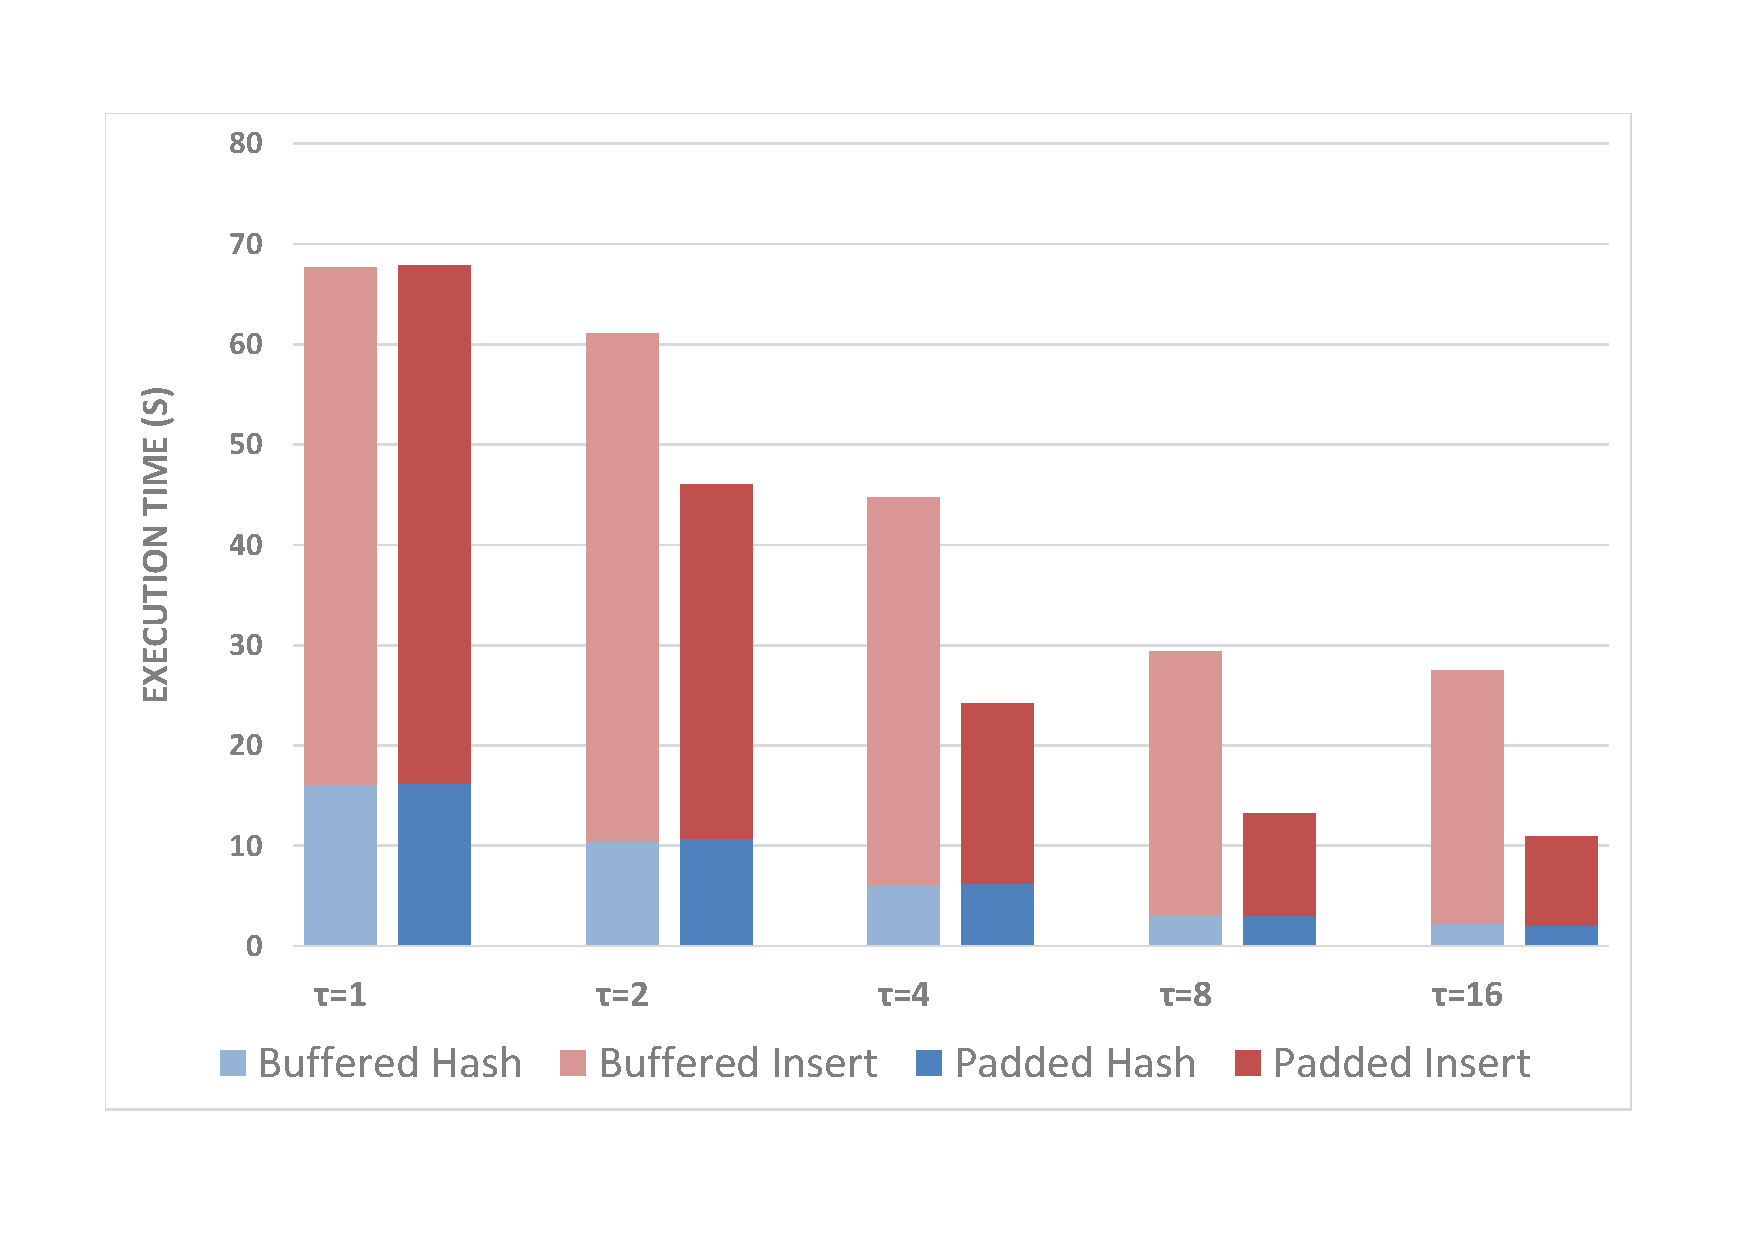
\includegraphics[width=\linewidth]{expfigs/8x211gandalf.pdf}
\caption{{\bf small} on {\bf Arch-1}}
\label{fig:8x211arch1}
\end{subfigure}
\begin{subfigure}[t]{0.45\textwidth}\hspace*{-10ex}
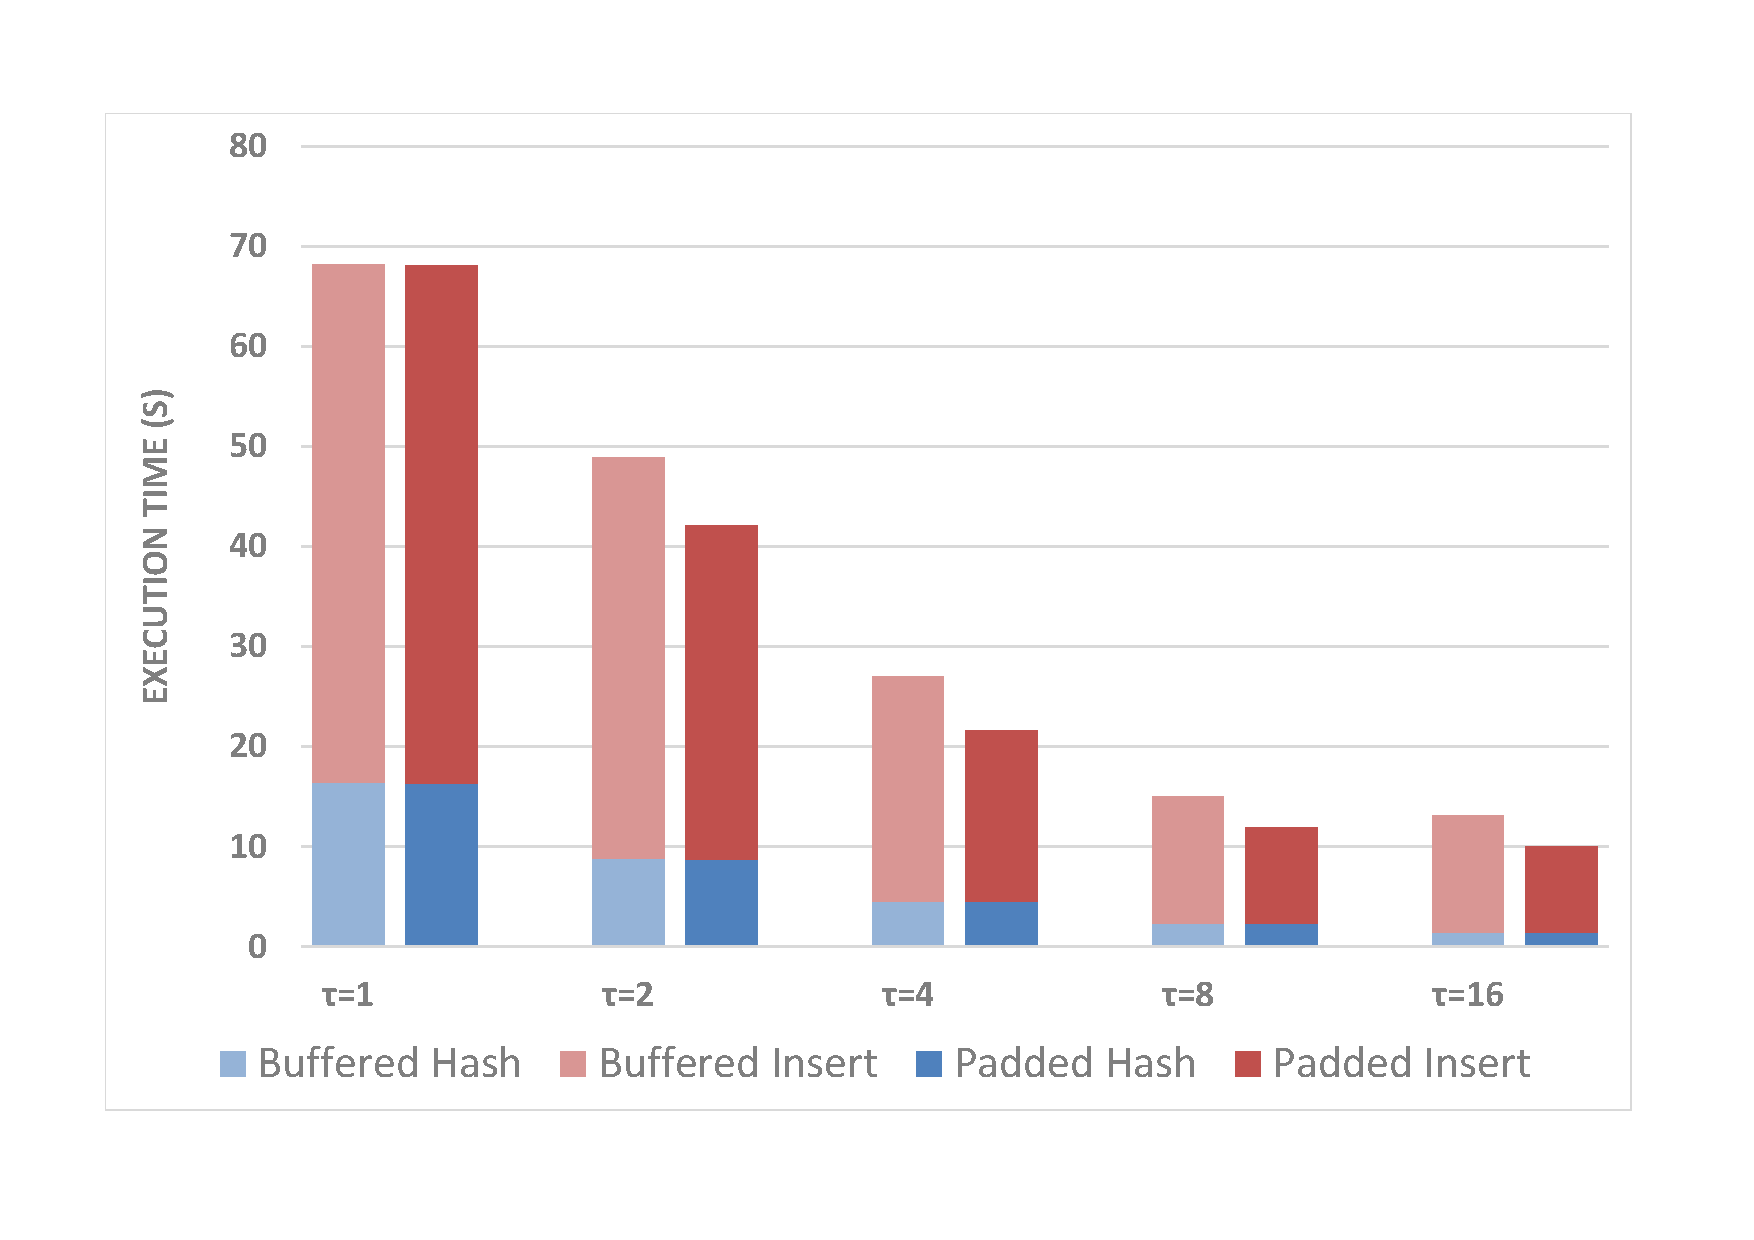
\includegraphics[width=\linewidth]{expfigs/8x2003gandalf.pdf}
\caption{{\bf large} on {\bf Arch-1}}
\label{fig:8x2003arch1}
\end{subfigure}
\begin{subfigure}[t]{0.45\textwidth}
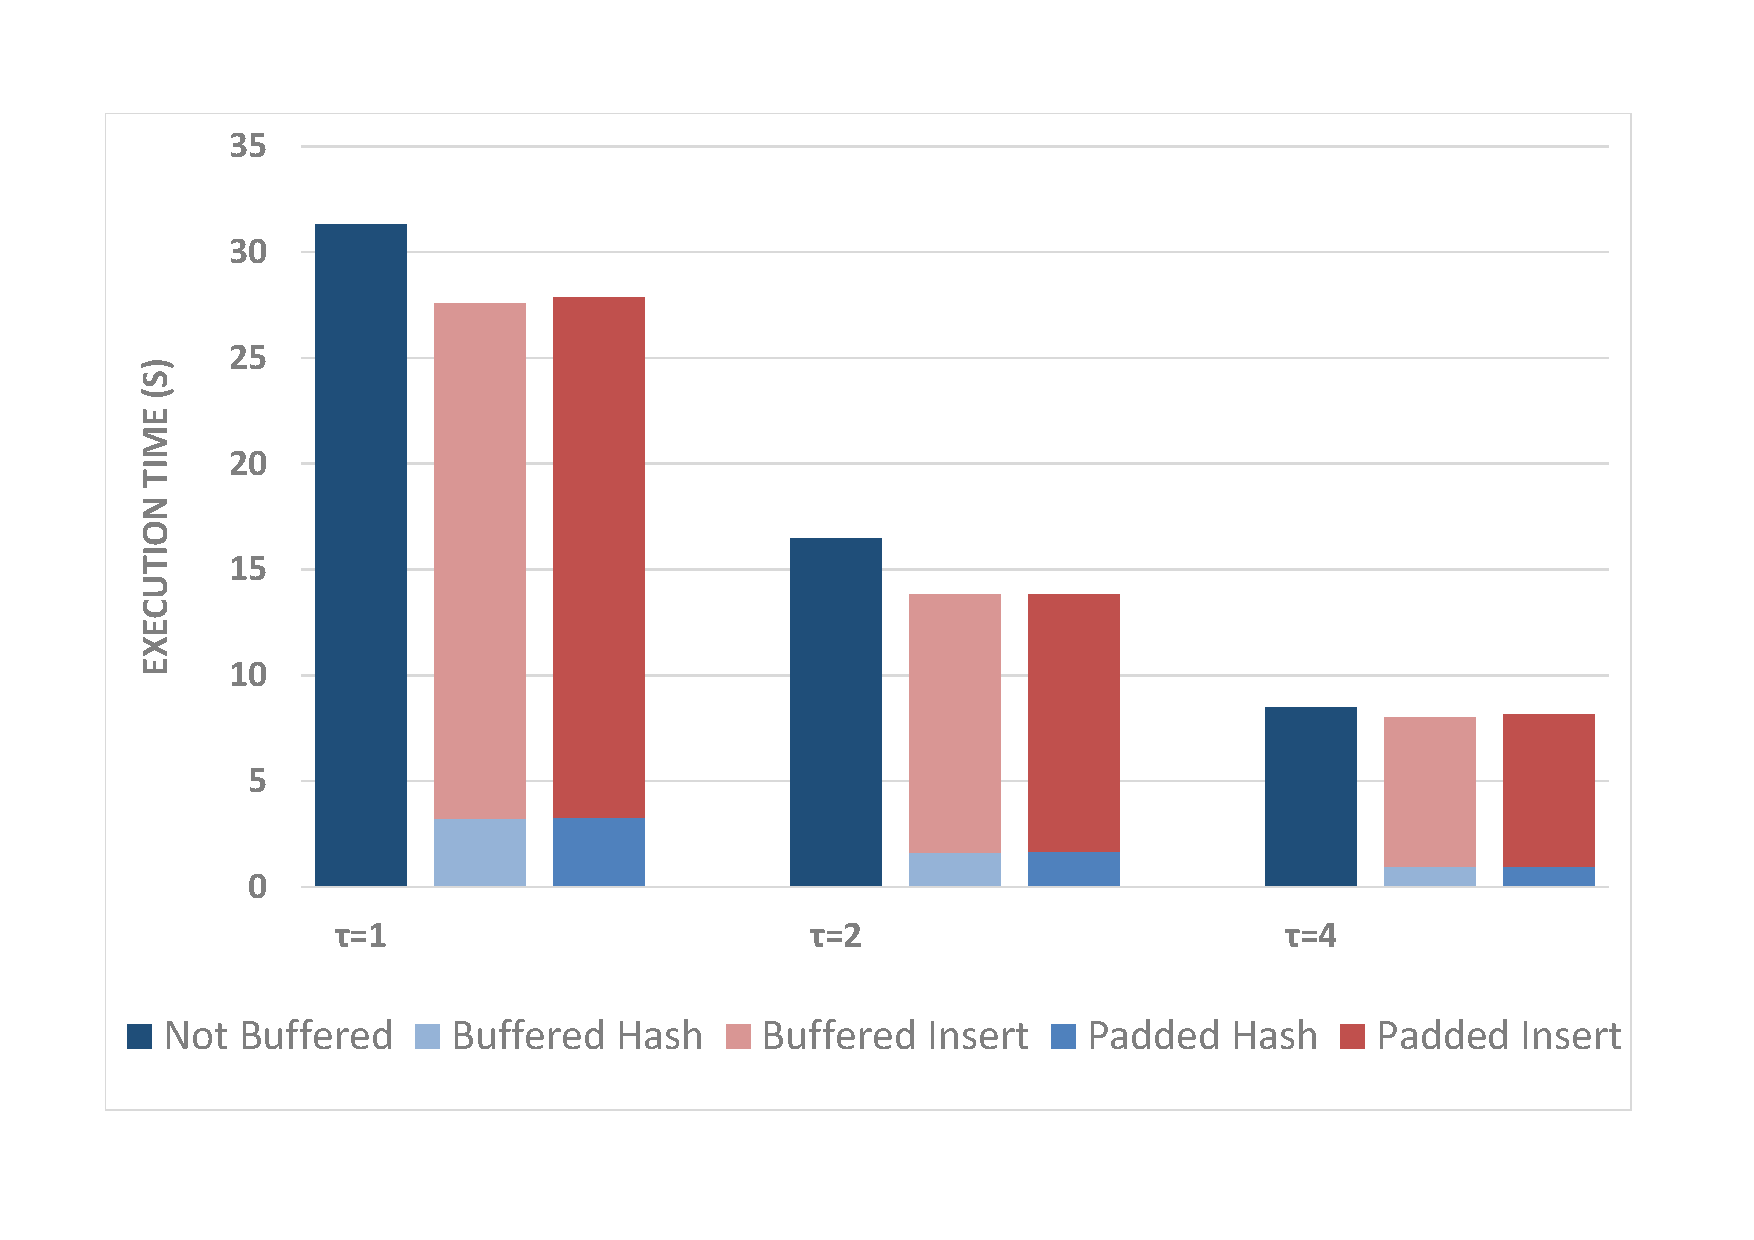
\includegraphics[width=\linewidth]{expfigs/8x211rasbpi.pdf}
\caption{{\bf small} on {\bf Arch-2}}
\label{fig:8x211arch2}
\end{subfigure}
\begin{subfigure}[t]{0.45\textwidth}\hspace*{2ex}
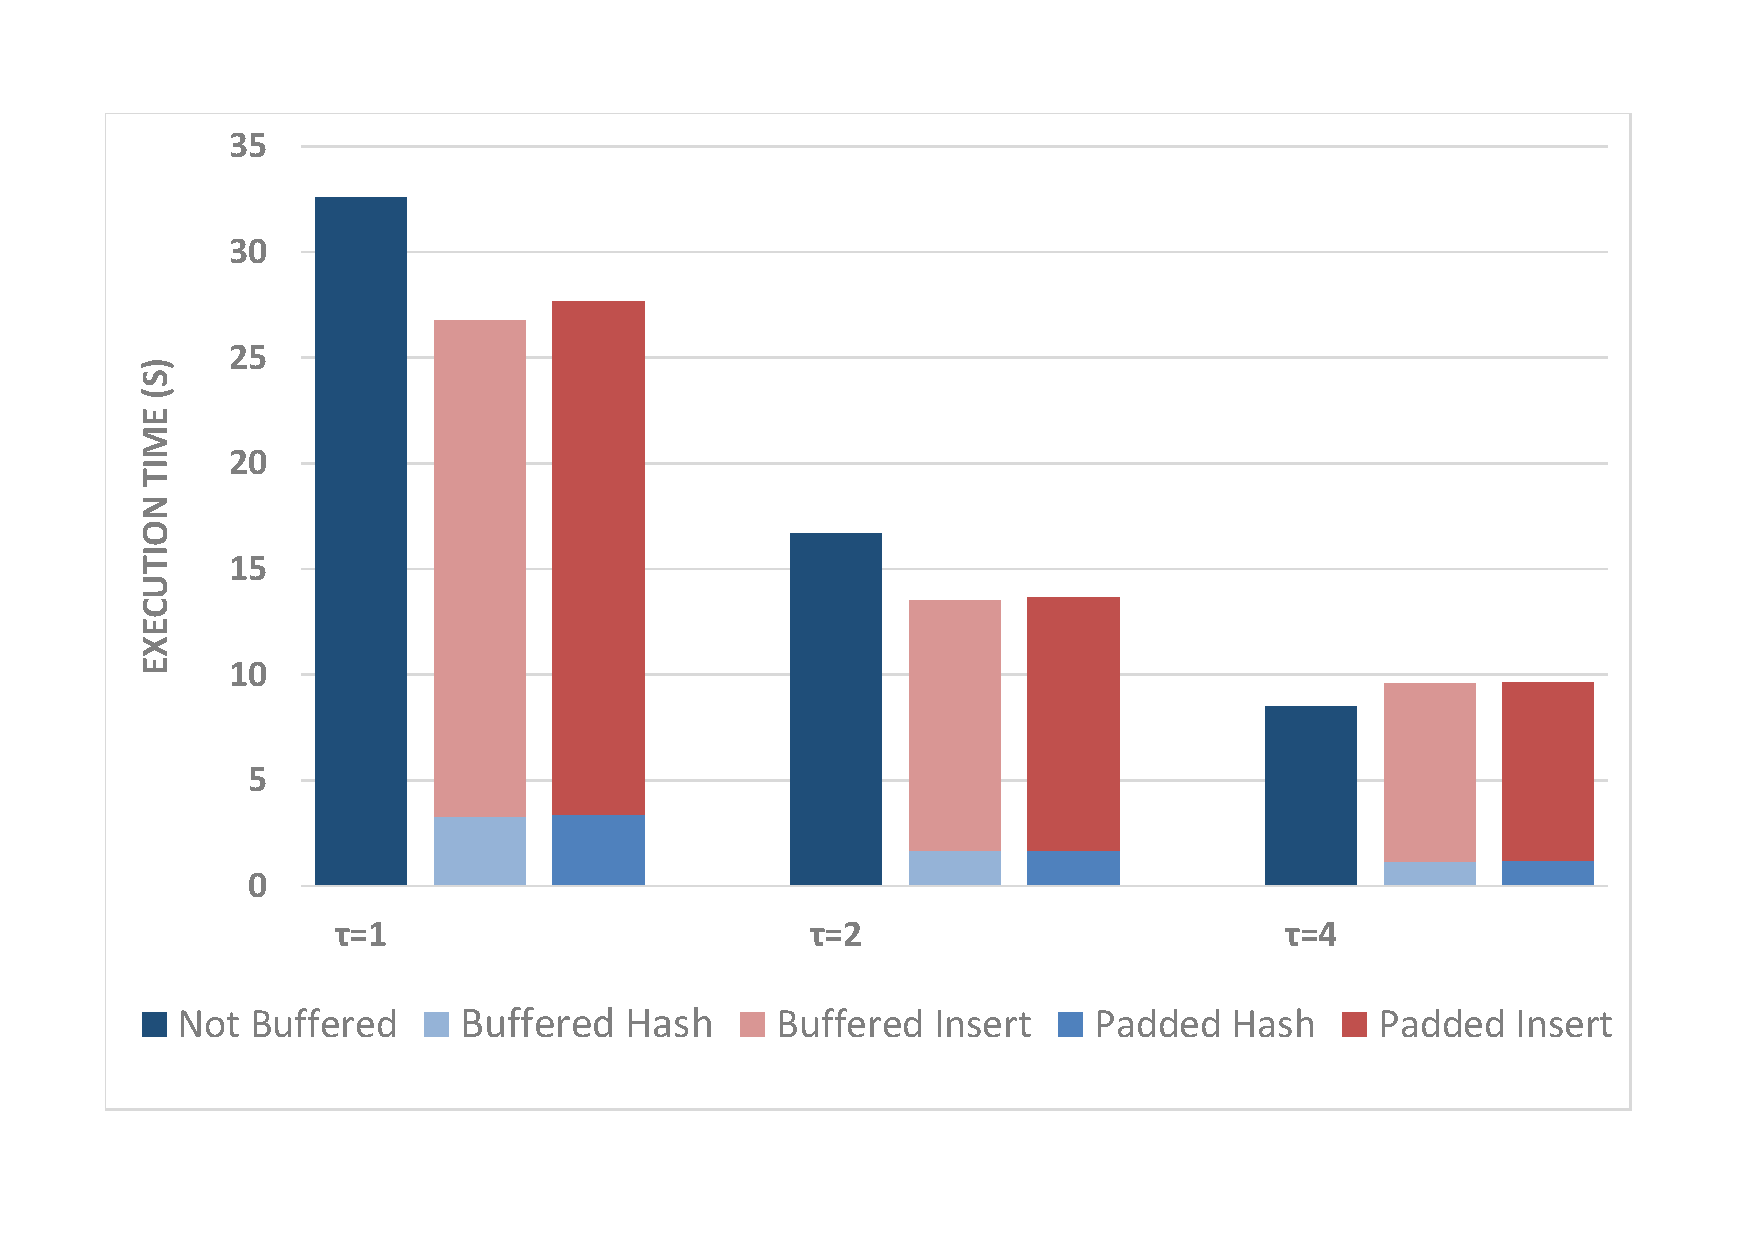
\includegraphics[width=\linewidth]{expfigs/8x2003rasbpi.pdf}
\caption{{\bf large} on {\bf Arch-2}}
\label{fig:8x2003arch2}
\end{subfigure}

\caption{Execution times (in seconds) for hashing and update/insertion stages for single CMS sketch experiments. The execution times for the naive parallel approach are omitted for {\bf Arch-1} since they are relatively much larger and deteriorate the visibility of the improvements.}
\label{fig:sum}
\end{figure*}

\subsection{Other optimizations}

In Algorithm~\ref{alg:cms_construct_par}, there is an implicit barrier between the first and second stages of the buffered parallel construction. This barrier guarantees that the buffer is filled and ready to be processed. For our experiments, we removed this barrier and implemented the buffered algorithms with OpenMPs {\tt nowait} directive. Although this may have a negative impact on the accuracy, when $b$ is large, the probability of a thread using a buffer entry which is not correctly set is small. Hence, we opt to remove the barrier. As Table~\ref{tbl:barrier} shows, this has a positive impact on the performance. To remove the threat to validity of the experiments, we measured how much we lost from the accuracy. Figure~\ref{fig:err} show the differences on the estimations for multithreaded executions compared to a single thread execution. The most frequent 1000 items are used for both charts in the figure. As the charts show, the differences are negligible considering that the real frequencies are in the order of tens of thousands for both cases.   
etween 
\begin{table*}[htbp]
	\centering
	{\def\arraystretch{1.3}
		\begin{tabular}{ccccc||ccccc|ccccc}  
			&&&&                 & \multicolumn{5}{c|}{\textbf{Buffered Parallel with Padding}} & \multicolumn{5}{c}{\textbf{Buffered Parallel with Padding + Barrier}} \\
			&&&&                 & $\tau$=1   & $\tau$=2    & $\tau$=4    & $\tau$=8    & $\tau$=16  & $\tau$=1   & $\tau$=2   & $\tau$=4   & $\tau$=8   & $\tau$=16 \\ \hline
			
			
			\multicolumn{1}{l}{\multirow{4}{*}{\textbf{Zipf 0.9}}}
			&&&\multirow{2}{*}{\textbf{Arch-1}} & \textbf{small}  & 68.3    & 46.7   & 24.4   & 13.6   & 10.9   & 69.0    & 44.7    & 23.8   & 13.7   & 11.2   \\
			&&&& \textbf{large} & 68.5    & 43.6   & 22.7   &   12.7 & 10.4   &  68.7 &	44.7 &	24.2	& 13.8	& 11.29 \\ \cline{2-15}
			
			&&&\multirow{2}{*}{\textbf{Arch-2}} & \textbf{small}  & 27.8    & 13.8   & 7.5   &        &       &  27.9    &  13.8   & 8.0   &        &       \\
			&&&& \textbf{large} &  27.2      &   13.3     &       8.3 &        &       &     27.6   &     13.6    &     9.3   &        &   \\ \hline  
			\multicolumn{1}{l}{\multirow{4}{*}{\textbf{Zipf 1.1}}}
			&&&\multirow{2}{*}{\textbf{Arch-1}} & \textbf{small}  & 68.09    & 43.5   & 22.9   & 13.0   & 10.6   & 68.2    & 45.6    & 24.6   & 14.2   & 11.5   \\
			&&&& \textbf{large} & 68.4    & 46.4   & 24.3   &   13.6 & 10.8   &  68.3 &	44.7 &	24.1	& 13.8	& 11.3 \\ \cline{2-15}
			
			&&&\multirow{2}{*}{\textbf{Arch-2}} & \textbf{small}  & 27.8    & 13.9   & 7.4   &        &       &  27.9    &  13.8   & 7.8   &        &       \\
			&&&& \textbf{large} &  27.1      &   13.3     &       8.1 &        &       &     27.5    &     13.5    &     9.3   &        &   \\ \hline  
			
				\multicolumn{1}{l}{\multirow{4}{*}{\textbf{Zipf 1.5}}}
			&&&\multirow{2}{*}{\textbf{Arch-1}} & \textbf{small}  & 67.9    & 44.6   & 23.49   & 13.1   & 10.6   & 68.1    & 44.3    & 24.2   & 13.8   & 11.4   \\
			&&&& \textbf{large} & 68.0    & 43.7   & 23.1   &   13.0 & 10.5   &  68.3 &	44.2 &	23.6	& 13.6	& 11.0 \\ \cline{2-15}
			
			&&&\multirow{2}{*}{\textbf{Arch-2}} & \textbf{small}  & 27.3    & 13.7   & 7.0   &        &       &  27.3    &  13.7   & 7.0   &        &       \\
			&&&& \textbf{large} &  26.5      &   13.2     &       7.5 &        &       &     26.4    &     13.1    &     7.49   &        &   \\ \hline  
			
				\multicolumn{1}{l}{\multirow{4}{*}{\textbf{Zipf 2}}}
			&&&\multirow{2}{*}{\textbf{Arch-1}} & \textbf{small}  & 67.7    & 44.5   & 23.6   & 13.1   & 10.6   & 68.0    & 45.3    & 24.5   & 14.0   & 11.4   \\
			&&&& \textbf{large} & 68.0    & 43.7   & 23.1   &   13.7 & 10.5   &  67.9 &	47.5 &	26.5	& 15.5	& 12.1 \\ \cline{2-15}
			
			&&&\multirow{2}{*}{\textbf{Arch-2}} & \textbf{small}  & 27.4    & 13.7   & 7.29   &        &       &  27.59    &  13.7   & 8.1   &        &       \\
			&&&& \textbf{large} &  26.2      &   13.0     &       7.9 &        &       &     26.2    &     13.0    &     7.8   &        &   \\ \hline 

				\multicolumn{1}{l}{\multirow{4}{*}{\textbf{Zipf 3}}}
			&&&\multirow{2}{*}{\textbf{Arch-1}} & \textbf{small}  & 67.7    & 43.1   & 22.9  & 12.8   & 10.5   & 67.8    & 45.6    & 24.3   & 13.9   & 11.4   \\
			&&&& \textbf{large} & 68.1    & 44.4   & 23.1   &   13.1 & 11.2   &  67.9 &	44.8 &	23.9	& 13.7	& 11.2 \\ \cline{2-15}
			
			&&&\multirow{2}{*}{\textbf{Arch-2}} & \textbf{small}  & 27.3    & 13.7   & 7.2   &        &       &  27.6    &  13.7   & 8.2   &        &       \\
			&&&& \textbf{large} &  26.3      &   13.1     &       7.4 &        &       &     26.2    &     13.1    &     7.8   &        &   \\ \hline 
						
			\multicolumn{1}{l}{\multirow{4}{*}{\textbf{Uniform}}}
			&&&\multirow{2}{*}{\textbf{Arch-1}} & \textbf{small}  & 68.7    & 43.5   & 22.8   & 13.0   & 10.6   & 68.6    & 43.8    & 23.5   & 13.5   & 11.1   \\
			&&&& \textbf{large} & 68.7    & 45.0   & 23.2   &   13.0 & 10.6   &  68.8 &	44.0 &	23.7	& 13.6	& 11.1 \\ \cline{2-15}
			
			&&&\multirow{2}{*}{\textbf{Arch-2}} & \textbf{small}  & 28.3    & 13.9   & 8.8   &        &       &  28.7    &  14.3   & 10.4   &        &       \\
			&&&& \textbf{large} &  27.4      &   13.39     &       8.5 &        &       &     27.79    &     13.9    &     9.6   &        &   \\ %\hline  
		\end{tabular}
	}
\caption{Impact of removing the barrier between the stages of buffered parallel execution on performance. The first set of the columns is the same with the last set of columns in Table~\ref{tbl:batch}. The values in the table are in seconds.}
\label{tbl:barrier}
\end{table*}

\begin{figure*}[htbp]
\begin{center}
\begin{subfigure}[t]{\textwidth}
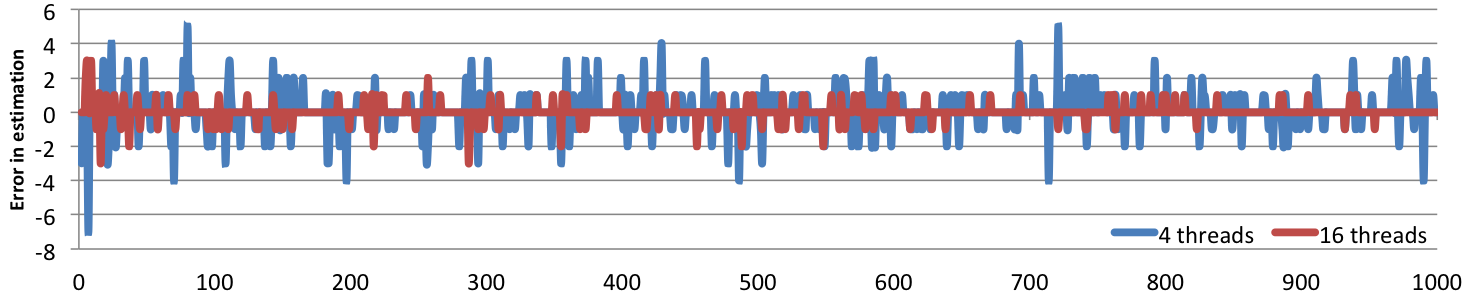
\includegraphics[width=\linewidth]{error1.png}
\caption{{\bf large} on {\bf Arch-1}}
\label{fig:err1}
\end{subfigure}
\end{center}

\begin{center}
\begin{subfigure}[t]{\textwidth}
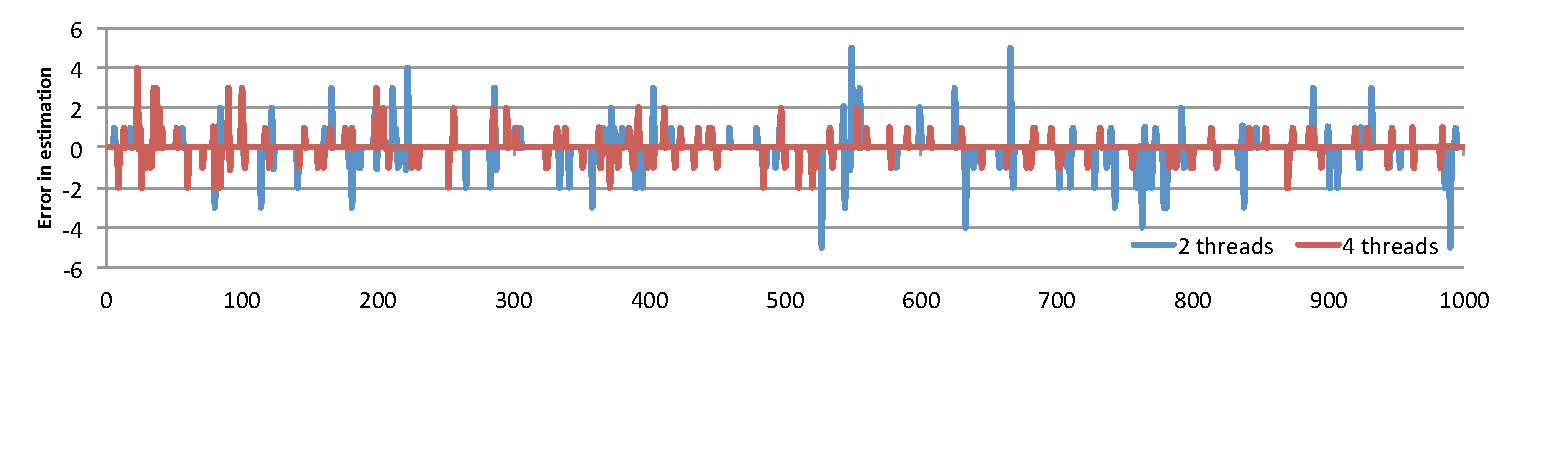
\includegraphics[width=\linewidth]{error2.pdf}
\caption{{\bf small} on {\bf Arch-2}}
\label{fig:err2}
\end{subfigure}
\end{center}

\caption{The difference between the frequency estimations of single and multithreaded executions of buffered parallel approach without the barrier. The charts show the differences for the top 1000 items for the {\bf large} sketch on {\bf Arch-1} and {\bf small} sketch on {\bf Arch-2}.}
\label{fig:err}
\end{figure*}

\section{Related Works}\label{sec:related}

CMS is proposed by Cormode and Muthukrishnan structure to summarize data streams~\cite{cormode2005} and it quickly became popular. They also suggest on sequential, parallel and hardware implementations of CMS~\cite{cormode2012} where the first parallel algorithm distributes rows to the threads so each thread computes the corresponding hash value. However, the hash computations are not merged as in our study. Another suggested algorithm is using multiple CMSs from different sub-streams and merge the results later.

Cafaro et al. propose an augmented frequency sketch for time-faded heavy hitters: recent items are considered to be more important~\cite{cafaro2016}. The authors extend this work via parallelization by dividing the stream into sub-streams and generating multiple sketches instead of a single one~\cite{cafaro2018}. When a query is issued, the result is computed using a reduce operation (as we did with multiple CMS tables in this study). There are studies in the literature employing synchronization primitives such as atomic operations for frequency counting~\cite{Das2009}. To the best of our knowledge, our work is the first cache-friendly, synchronization-free, single-table CMS algorithm specifically designed for limited-memory multicore architectures such as Raspberry Pi or other single-board computers. Furthermore, it utilizes tabular hashing which is recently shown to provide good statistical properties and reported to be fast~\cite{thorup2017,Dahlgaard2017}. When multiple hashes on the same item are required, which is the case for many sketches, our table-merging technique will be useful for algorithms using tabular hashing.

CMS has also been used as an underlying structure to design more advanced sketches. Recently, Roy et al. developed ASketch which filters high frequent items first and handles the remaining with a sketch such as CMS which they used for implementation~\cite{roy2016}. However, their parallelization depends on SPMD which stores multiple filters/sketches. Another advanced sketch employing multiple CMSs for parallelization is~\cite{Thomas2007}. If a single CMS sketch is neccesary, e.g., to fit into the cache, our techniques can be employed to develop more advanced parallel sketches using table-based ones such as CMS or Count Sketch.


\section{Conclusion}\label{sec:con}

In this work, we investigated parallelization of Count-Min Sketch on two multicore architectures; a high-end server and a single board computer. We proposed two main techniques. The first one, merged tabulation, is useful when a single is item needs to be hashed multiple times and can be used for different sketches and other applications performing the same task. The second technique is a classical one in high-performance computing, where the intermediate results are buffered to correctly synchronize the computation and regularize the memory accesses. The experiments we performed show that both techniques work for CMS construction on multicore architectures.

As a future work, we are planning to analyze the configuration options of the processors on single board computers such as how much data/instruction cache they use and how they handle coherency. Since sketches already incur inaccuracies, a freedom to have a little bit more can yield various optimizations. We also want to extend the architecture spectrum with other single board computers such as Odroid with heterogeneous cores and Parallela having many cores. We believe that similar techniques we develop here can also be used for other sketches. 

%Another thing we want to investigate is the impact of the distribution on the original data and devise a hybrid solution for different distributions. We stated the initial data distribution is not directly related with the execution time. However it can have an impact on the performance on for some applications where the stream contains only a few distinct items and hence, only a few counters are updated. This may increase the number of race conditions, and hence reduce the performance. However, when 



\bibliographystyle{IEEETrans}
\bibliography{sketch}
    
\end{document}
